% !TeX root = Protokoll.tex
\subsection{Absorption von $\gamma$-Strahlung}
\begin{figure}[h!]
	\centering
	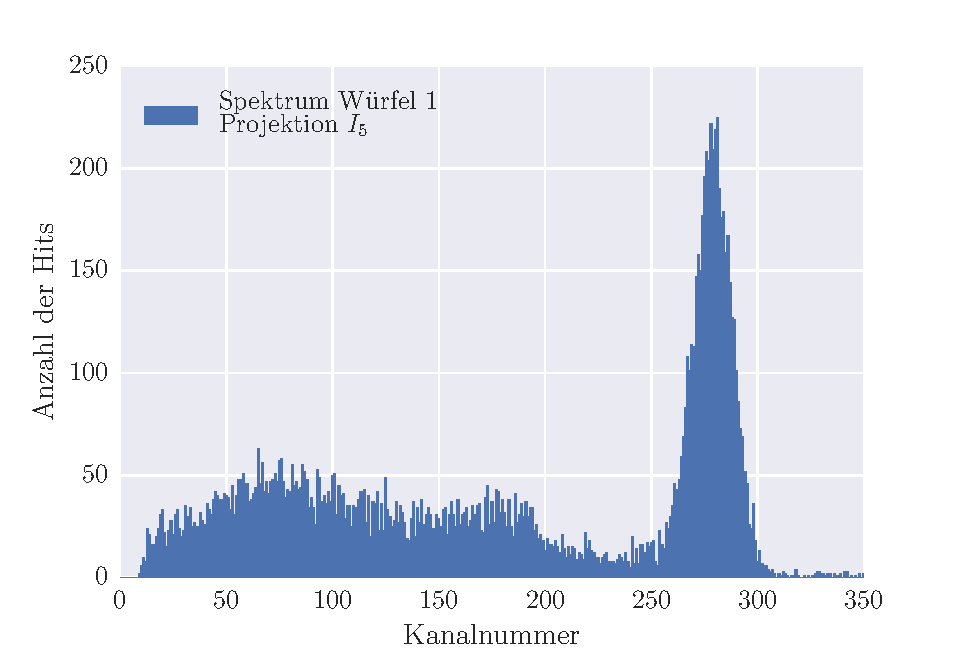
\includegraphics[width = 0.75\textwidth]{../Grafiken/Spektrum_Block_1_Messung_5_0_350_histogram.pdf}
	\caption{Ein aufgenommenes Energiespektrum von $\gamma$-Strahlung, nach Absorption durch eine Probe.}\label{fig:EnergieSpektrum}
\end{figure}
Wenn Strahlung auf Materie trifft, gibt es verschiedene Effekte wie sie miteinander wechselwirken. 
In diesem Versuch wird dabei mit $\gamma$-Strahlung gearbeitet.\\
Wenn $\gamma$-Strahlung mit Materie Wechselwirkt, tritt der Compton-, Photo-Effekt und mit genügend auch Paarbildung auf.
Bei dem Compton-Effekt streut ein Photon an einem Elektron und hat danach eine längere Wellenlänge.
Wenn ein Photon mit einer Energie, die mindestens so groß ist wie die Bindungsenergie des Elektrons auf ein Elektron trifft, gibt es seine Energie ab und das Elektron löst sich vom Atom.
Bei noch höheren Energien des Photons kann es, im Kernfeld, in ein Elektron Positron Paar Zerfallen.
In \cref{fig:EnergieSpektrum} ist das Spektrum für die Verwendete Quelle dargestellt.  
\newpage
\subsection{Verfahren der Tomographie}
Bei der Tomographie wird ein Objekt von mehreren Seiten bestrahlt und die Intensität der abgeschwächten Strahlung gemessen.
Daraus entsteht ein mehrdimensionale Darstellung des bestrahlten Objektes.
Dies resultiert daraus, dass die Strahlung in unterschiedlichen Materialien unterschiedlich stark abgeschwächt werden, weil sie nicht den selben Absorptionskoeffizienten $\mu$ besitzen.
\begin{wrapfigure}[16]{r}{0.5\textwidth}
	\centering
	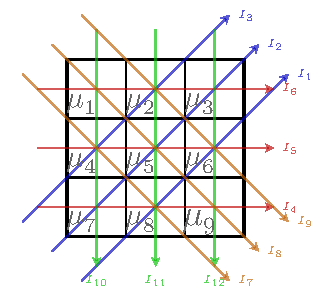
\includegraphics[width=0.5\textwidth]{../Grafiken/Tikz/tikz-Projektionen.pdf}
	\caption{Die Darstellung der Verwendeten Projektionen.\label{fig:Projektion}}
\end{wrapfigure}
In diesem Versuch wird dazu ein Würfel benutzt, der aus $3\times3\times3$ Elementarwürfeln besteht.
Die Intensität die durch verschiedene Stoffen abgeschwächt wird lässt sich dabei schreiben als
\begin{align}
	I = I_0e^{-\sum \mu_i d_i},
\end{align}
darin ist $I_0$ die maximal Intensität, $\mu_i$ der Absorptionskoeffizient des Materials und $d_i$ die in dem Material zurückgelegte Strecke. 
Daraus kann für die unterschiedlichen Projektionen $j$ mit den Ausgangsintensitäten $I_j$ geschrieben werden als
\begin{align}
	\sum \mu_j d_j = -\ln\left(\frac{I_j}{I_0}\right)=:N_j
\end{align}
\newpage
Diese Gleichung kann mithilfe von \cref{fig:Projektion} in eine Matrixdarstellung umgeschrieben werden.

\begin{align}
	d \cdot
	\underbrace{
	\begin{pmatrix}
		0 & 0 & 0  & 0 & 0 & \sqrt{2} & 0  & \sqrt{2} & 0\\
		 0&0  &\sqrt{2} & 0 & \sqrt{2} & 0 & \sqrt{2} & 0 & 0\\
		 0& \sqrt{2} & 0 & \sqrt{2} & 0 &0 &0  &0  &0 \\
		0&0 &0 &0 &0 &0 & 1 & 1 & 1\\
		0&0 &0 & 1 & 1 & 1 &0 &0 &0 \\
		1 & 1& 1 & 0&0 &0 &0 &0 &0\\
		0&0 &0 & \sqrt{2} & 0 &0 &0& \sqrt{2} &0\\
		\sqrt{2} & 0 & 0& 0 &\sqrt{2} &0 &0 &0 &\sqrt{2}\\
		0 & \sqrt{2} & 0 & 0 & 0 & \sqrt{2} & 0 & 0 &0\\
		1 &0 &0  &1 &0 &0 & 1 & 0 &0 \\
		0 & 1 & 0 & 0 & 1 & 0 & 0 & 1 &0 \\
		0 & 0& 1 & 0 & 0 & 1 & 0 & 0 & 1
	\end{pmatrix}
	}_{A}
	\cdot
	\underbrace{
	\begin{pmatrix}
		\mu_1\\
		\mu_2\\
		\mu_3\\
		\mu_4\\
		\mu_5\\
		\mu_6\\
		\mu_7\\
		\mu_8\\
		\mu_9
	\end{pmatrix}
	}_{\vec{\mu}}
	=
	\underbrace{
	\begin{pmatrix}
		N_1\\
		N_2\\
		N_3\\
		N_4\\
		N_5\\
		N_6\\
		N_7\\
		N_8\\
		N_9		
	\end{pmatrix}
	}_{\vec{N}}\nonumber
\end{align}
\begin{align}	
	\Rightarrow d \cdot A\cdot\vec{\mu}=\vec{N}
\end{align}
Weil $A$ eine $12\times 9 $ ist, wird daraus
\begin{align}
	\vec{\mu}=\frac{1}{d}\left(A^TA\right)^{-1}\cdot A^T\cdot\vec{N},
		\label{eq:KleinsteQuadrate}
\end{align}
dabei ist $d$ die Kantenlänge eines Elementarwürfels.
Der Fehler des $\vec{N}$ ist dabei durch eine Matrix gegeben durch
\begin{align}
	V[\vec{N}]=
	\begin{pmatrix}
		\sigma^2_{N_1} &  & 0\\
		 & \ddots & \\
		0 &  &\sigma^2_{N_{12}}	
	\end{pmatrix}.
\end{align}
Daraus ergibt sich die Kovarianzmatrix zu
\begin{align}
	V[\vec{\mu}]=\left(A^TV^{-1}[\vec{N}]A\right)^{-1}
\end{align}
und $\vec{\mu}$ muss dann umgeschrieben werden zu
\begin{align}
	\vec{\mu}=\frac{1}{d}V[\vec{\mu}]\cdot A^T V^-1[\vec{N}] \vec{N}
\end{align}
\newpage
